\scanpage{142}
$\mathbb R_!f(L_\bullet)$ est de Tor-dim. majorée par
$[N-2d\deleted{\unsure{'}},M\deleted{\unsure{+2d}}]$. (notations \deleted{\unsure{hom}} de degrés \uline{inférieurs}!)

Résulte \unsure{formellt} de Künneth: on a
\[
\mathbb R_!f(L_\bullet)\overset{\mathbb L}{\otimes}\deleted{\unsure{M}}L'_\bullet\simeq\mathbb R_!f(L_\bullet\otimes\mathbb Lf^*(L'_\bullet)\unsure{.})
\]
si
$L'_\bullet$ est de \inserted{ch. \unsure{de}} dim majorée par $[N',M']$,
$\mathbb Lf^*(L'_\bullet)$ itou, $L_\bullet\otimes\mathbb Lf^*(L'_\bullet)$ est à ch. de
degrés majorés par $[N+N',M+M']$, donc
$\mathbb R_!f(\qquad)$ est à ch. de degrés bornés par
\[
[N+N'-2d,M+M'],
\]
(notation homologique!)
ce qui est la relation qu'on voulait prouver.
\figure{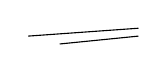
\begin{tikzpicture}\draw (0,0)--(1.4,.1);\draw (.4,-.1)--(1.4,0);\end{tikzpicture}}
\deleted{Soit maintenant $A$ un anneau commutatif,
que nous supposerons artinien pour simplifier.
Considérons}
\figure{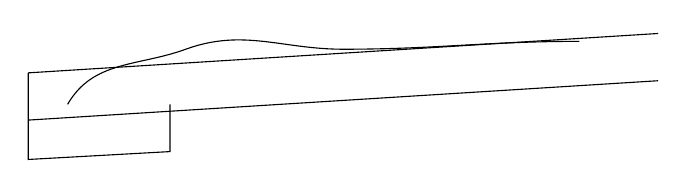
\begin{tikzpicture}\draw (0,0)--(8,.5);\draw (0,-.6)--(8,-.1);\draw (0,0)--(0,-1.1)--(1.8,-1)--(1.8,-.4);\draw (.5,-.4) to[out=60,in=200] (2,.3) to[out=20,in=180] (4,.3) to[out=0,in=180] (7,.4);\end{tikzpicture}}
\mspage{141}
